%                                                                 aa.tex
% AA vers. 9.2, LaTeX class for Astronomy & Astrophysics
% Demonstration file
%                                                       (c) EDP Sciences
%-----------------------------------------------------------------------
%
%\documentclass[referee]{aa}    % for a referee version
%\documentclass[onecolumn]{aa}  % for a paper on 1 column  
%\documentclass[longauth]{aa}   % for the long lists of affiliations
%\documentclass[letter]{aa}     % for the letters
%\documentclass[bibyear]{aa}    % if the references are not structured
                                % according to the author-year natbib style

\documentclass{aa}

\usepackage{graphicx}     
\usepackage{txfonts}      
\usepackage{lipsum}      
\usepackage{subcaption}   
\usepackage{lscape}      
\usepackage{placeins}     
\usepackage{natbib}     

\usepackage{hyperref}     

\usepackage{caption}
\captionsetup{compatibility=false}

%%%%%%%%%%%%%%%%%%%%%%%%%%%%%%%%%%%%%%%%
%\usepackage[options]{hyperref}
% To add links in your PDF file, use the package "hyperref"
% with options according to your LaTeX or PDFLaTeX drivers.
%%%%%%%%%%%%%%%%%%%%%%%%%%%%%%%%%%%%%%%%

% - use BibTeX with the regular commands:
%\bibliographystyle{aa} % style aa.bst
%\bibliography{myBib.bib} % your references Yourfile.bib

%
% - join the .bib files when you upload your source files
%-------------------------------------------------------------------

\begin{document}

   \title{Review: SHOTGLAS II}

   \subtitle{MUSE spectroscopy of blue horizontal branch stars in the core of Centauri and NGC 6752 \thanks{The original paper is from \citep{2023A&A...677A..86L}}}

   \author{A. V\"olkerer\inst{1}
        }

   \institute{University of Vienna, Department of Astrophysics, T\"urkenschanzstrasse 17, 1180 Vienna, Austria\\
             \email{a12313738@unet.univie.ac.at} \\
             Student ID number: 12313738}

   \date{Submission date: February 7, 2025}

% \abstract{}{}{}{}{}
% 5 {} token are mandatory
 
  \abstract
  % context heading (optional)
  % {} leave it empty if necessary  
   {For the WSP course, it is required to write a paper in the A\&A style. }
  % aims heading (mandatory)
   {In this paper I aim to provide a review of the paper \cite{2023A&A...677A..86L}. The paper \cite{2023A&A...677A..86L} analyzed horizontal branch stars from centers of globular clusters. They used $\omega$ Centauri and NGC 6752. They compared their observations with models.}
  % methods heading (mandatory)
   {They used MUSE spectroscopy and HST photometry to observe the data. Synthetic spectra was calculated with a hybrid LTE/NLTE modeling approach. This approach describes the stars atmosphere, some parameters are obtained. These parameters were compared. Further, with the LTE/NLTE model a spectral energy distribution (SED) was calculated. With the SEDs other parameters are calculated and were also compared.}
  % results heading (mandatory)
   {For stars with a temperature lower 15000 K, the theoretically results are good. For warmer stars another model or other input parameters are needed. }
  % conclusions heading (optional), leave it empty if necessary
   {It was showed, that the combination of MUSE spectra and HST photometry is powerful. It presents various methods for deriving the properties of stars and globular clusters.}

   \keywords{review --
                stars: fundamental parameters,
                stars: horizontal-branch,
                globular clusters: individual: NGC5139,
                globular clusters: individual: NGC6752,
                          }

   \maketitle


%%%%%%%%%%%%%%%%%%%%%%%%%%%%%%%%%%%%%%%%%%%%%%%%%%%%%%%%%%%%%%

\section{Introduction}
\label{sec:1}
The goal of this paper is to introduce you to the work presented in \cite{2023A&A...677A..86L}. First, I will explain the subject. Secondly, I will provide a brief summary of the most important techniques. In the original paper more subjects were discussed like: atmospheric parameters, variable stars and some other topics in detail. I will discuss them briefly or not at all. I believe these topics are too specific to provide a good overview of the paper and its techniques. When referring to the original paper, \cite{2023A&A...677A..86L} is referenced. 

Globular clusters (GC) are old star clusters. Star clusters contain stars with a familiar age, helium abundance, mass, metallicity and so on. Stars in clusters are gravitationally bound to the other stars. Many stars have left the main sequence ind GC. The main sequence is in a Hertzsprung-Russel diagram, where most of the stars are, this is the "main lifetime" of a star. The stars only fusses Hydrogen in the cores. If the corse do not contain enough Hydrogen to fusion, the next step in stellar evolution is reached. High mass stars (which were analyzed) enter the Horizontal Branch (HB). In this phase, the nucleus fuses helium. These stars were observed. This is important for the understanding of stellar evolution.

The paper \cite{2023A&A...677A..86L} used multiple data, from the Multi Unit Spectroscopic Explorer (MUSE) \citep{2010SPIE.7735E..08B}, at the Very Large Telescope (VLT) and the Hubble Space Telescope (HST), for more details, see Section \ref{sec:2}. They used a hybrid model to create synthesized spectra, this is discussed in Section \ref{sec:3}. From both spectra the effective temperature ($T_{\text{eff}}$), the surface gravitation ($\log{g}$) and the helium abundance were derived. The model was further used to fit a Spectral Energy Distribution (SED) to derive average reddening, radius, luminosity, and mass of the stars (the methods to determine these quantities would take too long). The model spectra and SEDs were compared with the observed spectra and SEDs. For more detail, see \ref{sec:3}. They compared the positions of the Momany-jump (M-jump) \citep{2002ApJ...576L..65M} and the Grundahl-jump (G-Jump) \citep{1999ApJ...524..242G}. For more detail see \ref{sec:4}. Their results were pretty good for stars at <15000 K, for more see \ref{sec:5}. 

\begin{figure*}
        \centering
        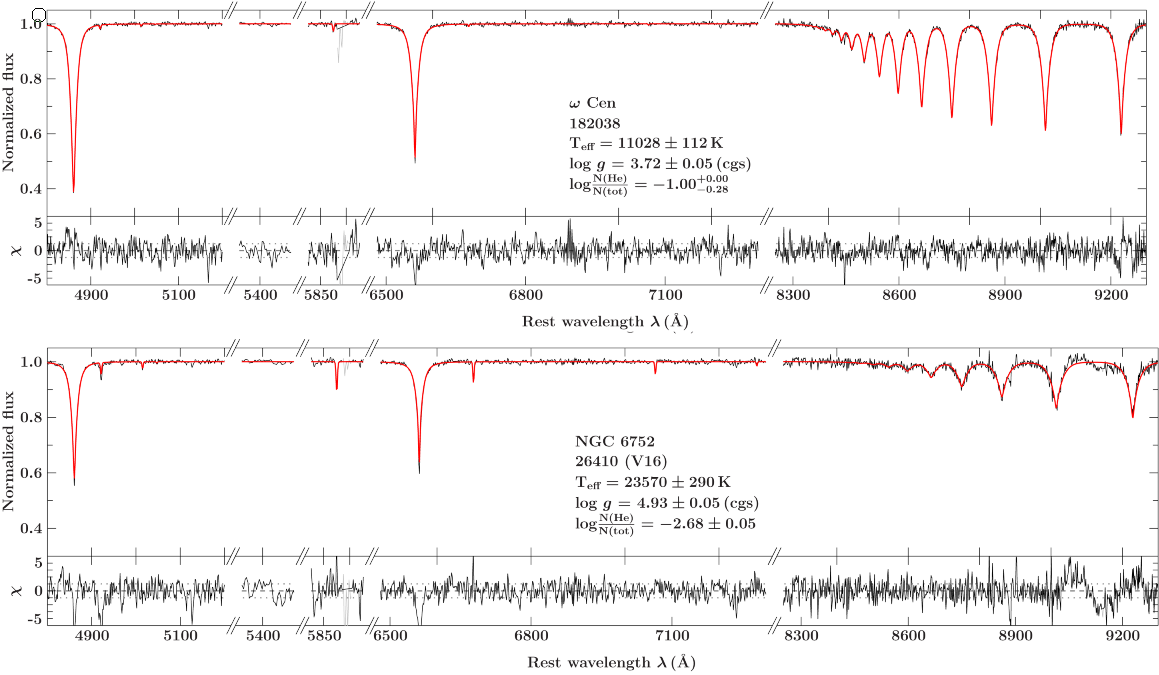
\includegraphics[width=\hsize]{fitSpecBearb.png}
        \caption{A part of the analyzed spectra. On the upper plot for $\omega$ Cen and on the lower for NGC 6752. On the x-axis is the wavelength in \AA ngstr\"om ($1 \text{\AA} = 0.1nm$). On the y-axis is the normalized flux of the spectra. The $\chi$ is the residual of each data point (see equation \ref{eq:chi}). I have edited the figure, the original figures is in \cite{2023A&A...677A..86L}, figure 4 and 5}
        \label{fig:Spec}
\end{figure*}

%%%%%%%%%%%%%%%%%%%%%%%%%%%%%%%%%%%%%%%%%%%%%%%%%%%%%%
\section{Data}
\label{sec:2}
They used $\omega$ Centauri ($\omega$ Cen/NGC 5139) and NGC 6752, because both globular Clusters are well known. But $\omega$ Cen have a wide range of metallicity and helium abundances. In contrast is NGC 6752, which is more homogeneous.  
For catalogs were used:

\begin{itemize}
\label{list:catalogs}
    \item The first catalog is HUGS (HST UV Globular Cluster Survey) from \cite{2015AJ....149...91P} and \cite{2018MNRAS.481.3382N}. HUGS provides photometric data in five filters from ACS/WFC and WFC3/UVIS. The HST were used.
    \item The second catalog is \cite{2017ApJ...842....6B}, it contains photometry in multiple WFC3/UVIS filters for $\omega$ Cen. The HST were used.

    \item The third catalog is \cite{2010ApJ...710.1032A}, it contains ACS/WFC F435W and F625W magnitudes for $\omega$ Cen.

    \item The fourth  cataloge is the MUSE GC Survey from \cite{2018MNRAS.473.5591K} it contains a spectroscopic dataset covering the core regions of $\omega$ Cen and NGC 6752, enabling radial velocity and stellar parameter measurements.
\end{itemize}

Only for the MUSE catalog were some information about the observation. The spectra covers 475-935nm (4750-9350\AA). With a spectral resolution of $R \sim 3000$. The spectra are extracted using the PAMPELMUSE software \citep{2013A&A...549A..71K, 2018MNRAS.473.5591K}. PAMPELMUSE do the analysis of integral-field spectroscopic observations \footnote{For a PAMPELMUSE user guid see: \href{https://pampelmuse.readthedocs.io/en/latest/index.html}{https://pampelmuse.readthedocs.io/en/latest/index.html}}. These spectra were fitted with the PHOENIX spectral library \cite{2013A&A...553A...6H}. PHOENIX generates synthetic stellar atmosphere spectra by solving the radiative transfer equations under both Local Thermodynamic Equilibrium (LTE) and Non-Local Thermodynamic Equilibrium (NLTE) conditions.


\begin{figure}
        \centering
        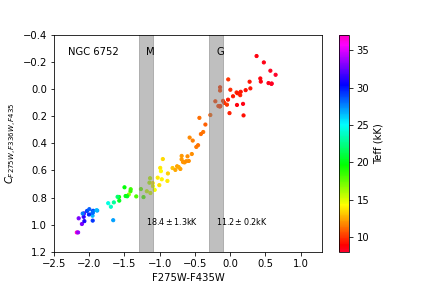
\includegraphics[width=\hsize]{NGC6752.png}
        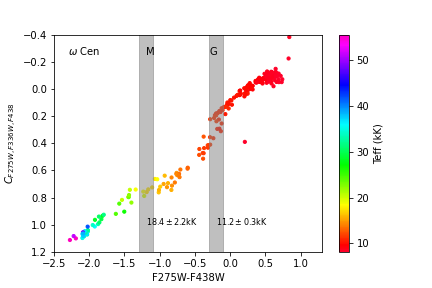
\includegraphics[width=\hsize]{wCen.png}
        \caption{In the upper plot the color-color diagram, for NGC 6752 can be seen and in the lower plot for $\omega$ Centauri. The positions of the jumps are highlighted. The temperatures are consistent with the literature. }
        \label{fig:C-C_self}
\end{figure}

%%%%%%%%%%%%%%%%%%%%%%%%%%%%%%%%%%%%%%%%%%%%%%%%%%%%%%
\section{Analysis method}
\label{sec:3}
To create synthetic spectra, a model for a star's atmosphere was created. The model is a ADS approach. ADS is a hybrid method of Local Thermal Equilibrium (LTE) and Non-Local Thermal Equilibrium (NLTE). This method was first described by \cite{2006A&A...445.1099P} and \cite{2007A&A...467..295N}. The first step of the approach is calculating the atmosphere in LTE with the ATLAS12 software \cite{1996ASPC..108....2K}. ATLAS12 can calculate the atmosphere in LTE. The advantage is that this program can calculate a atmosphere with individual abundances. The LTE atmosphere is one input parameter of DETAIL \citep{1981PhDT.......111G}. DETAIL calculates the population of hydrogen and helium atoms in NLTE (step 2).  These data are the new input data for ATLAS12 (step 1). The new data are given into DETAIL and so on (step 2). Until the numbers are convergent. Then comes SURFACE \citep{1981PhDT.......111G}. SURFACE calculates the synthetic spectra, with the population, which was calculated with DETAIL. 

The result can be seen in figure \ref{fig:Spec}. In \cite{2023A&A...677A..86L} both spectra have a longer range, from $\approx 4900 - 9200 \text{\AA}$ for both GC. The black line is the normalized observed spectra and the red line is the fit. Only the hydrogen and the helium lines are displayed. The $\chi$ are the residuals. The residuals are the differences between the observed value and the expected / fitted value. In some cases is the residual divided by the variance of the observed data $\sigma_\text{observed}$. This is done to get a weighing of the residuals. The paper did not mention which definition they have choose, but I assume the weighing, because of the values in the plot. In this case is $\chi_i$ is the residual error ($\chi_i$ residual for the i-th data point). The residual formula can be seen in equation \ref{eq:chi}. 

\begin{equation}
\label{eq:chi}
\chi_i = \frac{F_\text{i, Observed}-F_\text{i, Fit}}{\sigma_\text{i, Fit}}
\end{equation}

The chi-squared test can be performed using the residual error. This test check how well the model perform, it "describes the goodness-of-fit". In equation \ref{eq:chiSqu} the distribution can be seen. 
\begin{equation}
\label{eq:chiSqu}
\chi^2 = \sum_{i=1}^n \frac{F_\text{i, Observed}-F_\text{i, Fit}}{\sigma_\text{i, Fit}}
\end{equation}
To get the probability, for a significance level $\alpha$, the value of chi squared Sitributioen can be read in a table. Or the compute do everything 

This was a small step of the whole work. They also discussed how the SED were fitted, the treatments of helium and the treatments of metallicity. 

%%%%%%%%%%%%%%%%%%%%%%%%%%%%%%%%%%%%%%%%%%%%%%%%%%%%%%

\section{M-jump and G-jump}
\label{sec:4}
In this Section, I have done some data analysis. Perhaps some incorrect analysis tools, methods, or misunderstandings were used. All of the files can be found at \href{https://github.com/MonkeyTreeLover/MiniPaper_WSP}{https://github.com/MonkeyTreeLover/MiniPaper\_WSP}. The data, which I used is from the orignial paper published on Vizier. 

The Momany jump (M-jump) \citep{2002ApJ...576L..65M} and the Grundahl jump (G-jump) \citep{1999ApJ...524..242G} can be seen in color-color diagrams. The jumps can only occur in HB stars. The jumps are rapid changes in the spectra of the stars. This change can be seen in the figure \ref{fig:C-C_self}. Both jumps occur during the phase of the HB of a star. With these jumps, the age / state of the star can be determined. \\
The G-jump occurs first, at a temperature about 11.5 kK (in the paper at 11.2 kK). This occurs when radiative levitation is stronger than the gravitational force. As a result, some metals are transported into the stars atmosphere and the spectra that we observe change.  \\
The M-jump occurs at a temperature about 20 kK (in the paper 18.4kK). At the temperature, the hydrogen ionizes at the stars atmosphere. This causes change in the spectra. 

The color index is a measure of a star's color. This is the definition of the color index $C_{F275W, F336W, F435W} = (m275W-m336W)-(m336W-m435W)$. The same approach is used for the other color index $C_{F275W, F336W, F438W} = (m275W-m336W)-(m336W-m438W)$. This equation was first used by \cite{2013ApJ...767..120M}, on page 3 in Section 3. 
To determine the temperatures of the two jumps, their positions in the color-color diagram were identified. For the M-jump in NGC 6752 this position were taken $F275W-F435W=-1.2 \pm 0.2$. The mean temperature of the stars in range were calculated. The result is $18.4 \pm 1.3 kK$. The same procedure were made for the G-jump with $F275W-F435W=-0.2 \pm 0.2$. For $\omega$ Cen the same procedure were made for the M-jump: $F275W-F348W = -1.2 \pm 0.2$,  and for the G-jump; $F275W-F438W = -0.2 \pm 0.2$. The diagrams were done by me, but i have not done the determination of the temperatures. 

\begin{figure}
        \centering
        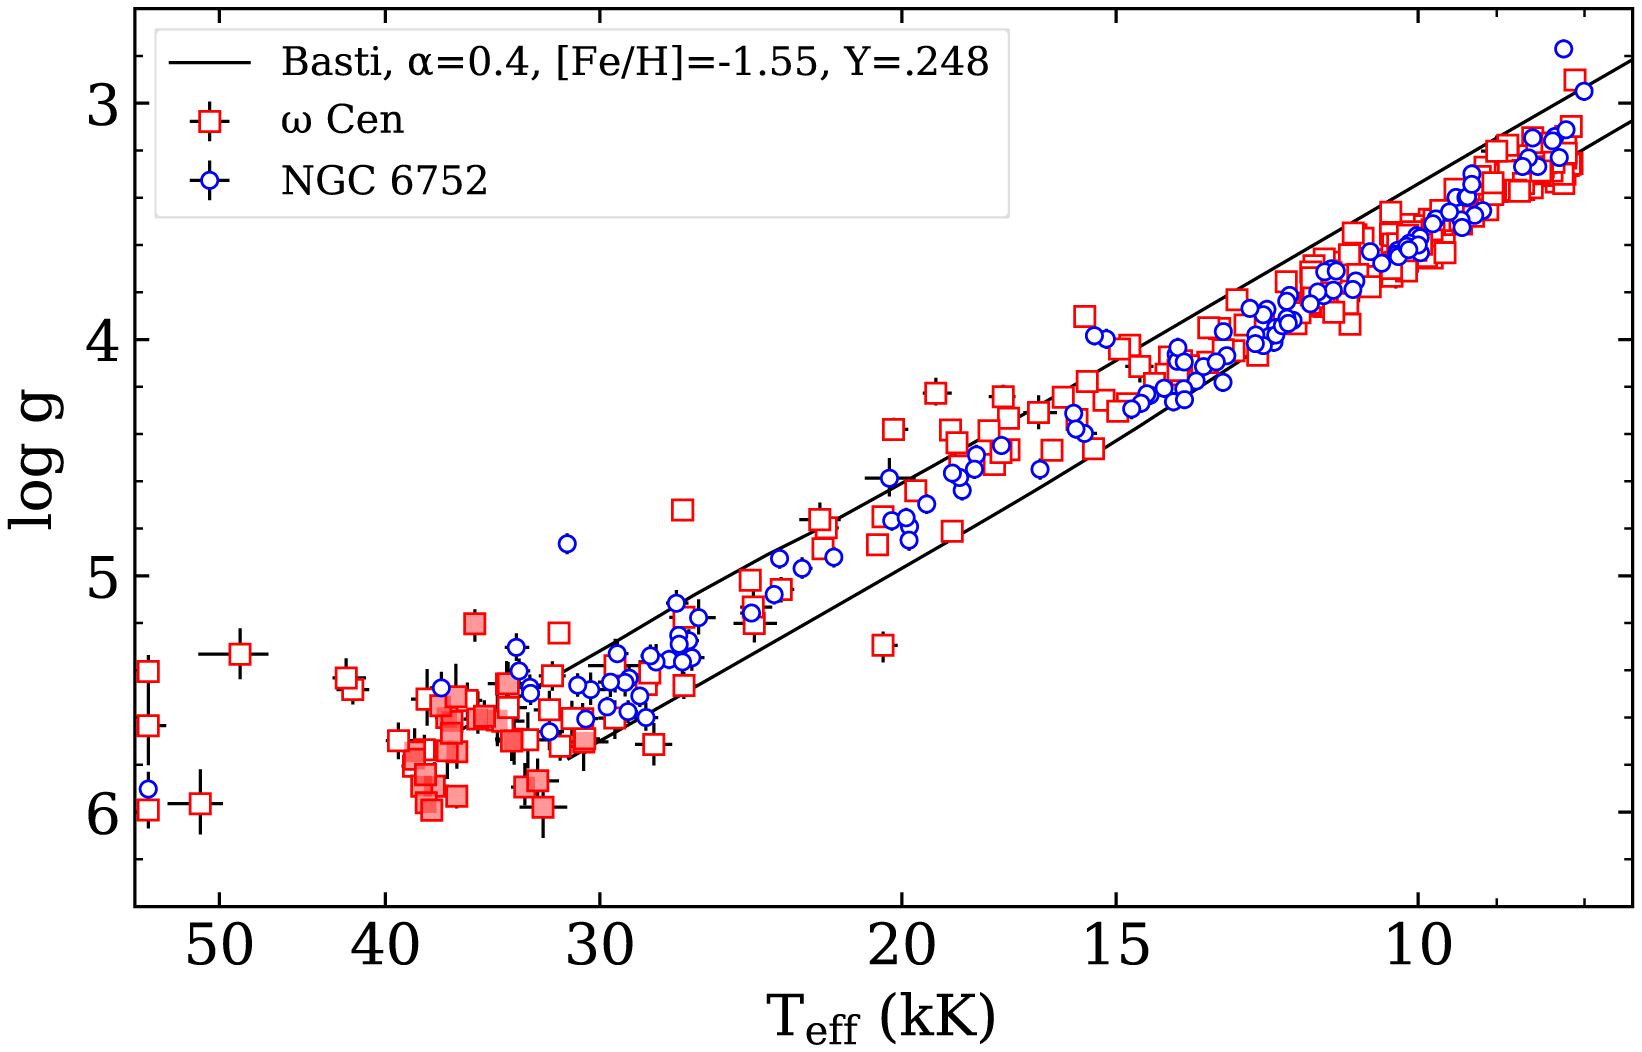
\includegraphics[width=\hsize]{prediction.png}
        \caption{This figure compares the data and the model, for $T_\text{eff}$ and $\log g$. Stars from $\omega$ Cen are red squares. Stars from NGC 6752 are blue circles. The black line is the predicted model. This diagram is in \cite{2023A&A...677A..86L} figure 15. Similar plots can be seen in figure 14 and 16.}
         \label{fig:prediction}
\end{figure}

%%%%%%%%%%%%%%%%%%%%%%%%%%%%%%%%%%%%%%%%%%%%%%%%%%%%%%%%%%%%%%
\section{Results}
\label{sec:5}
Not only the spectra and SEDs were analyzed, but also the quantities derived from them. The quantities are: effective temperature ($T_\text{eff}$), surface gravitation ($\log g$), radius ($R$), luminosity ($L$) and mass ($M$). Diagrams were created, on the x-axis is $T_\text{eff}$ and on t y-axis another parameter ($\log g$, $R$, $L$ or $M$). In figure \ref{fig:prediction} such a diagram can be seen. For temperatures above approximately 15,000 K, the model is good. There is no significant difference between $\omega$ Cen and NGC 6752. For the other diagrams (not shown in this paper), the results are familiar. 
Although the two clusters have different spreads of metallicity, no significant difference could be found. Only for the variable stars and Blue Strangler Stars

%%%%%%%%%%%%%%%%%%%%%%%%%%%%%%%%%%%%%%%%%%%%%%%%%%%%%%%%%%%%%%
\section{Conclusions}
\label{sec:6}
The original paper analyzed HB stars from $\omega$ Cen and NGC 6752. They used HST photometry and MUSE spectroscopy  (see \ref{list:catalogs}). They used a hybrid LTE/NLTE modeling approach, to get a synthetic atmosphere and its spectra and photometry. Some quantities were derived from the observed data and from the fitet data. No significance differences were found between both GC. The model is valid for temperatures above 15 kK. 
The author mentioned as future work, differnt GC to analyze, improving the models and investigate the evolution of HB stars. 
I have provided some information about what data was used \ref{list:catalogs}. The process of creating the synthetic spectra were discussed and how to fit it with the observed data. The importance of the M-jump and G-jump and how they are created. The process of determination of the temperature were discussed in detail and two color-color diagrams are made \ref{fig:C-C_self}. Then the results and differences between both GC were discussed.

%%%%%%%%%%%%%%%%%%%%%%%%%%%%%%%%%%%%%%%%%%%%%%%%%%%%%%%%%%%%%%
\begin{acknowledgements}
      I want to thank the team of the paper \citep{2023A&A...677A..86L}. For writing the paper I used OVERLEAF (\href{https://www.overleaf.com/}{https://www.overleaf.com/}). For the image processing I used KRITA (\href{https://krita.org/en/}{https://krita.org/en/}). This review has made use of NASA's Astrophysical Data System Bibliographic Services (\href{https://ui.adsabs.harvard.edu/}{https://ui.adsabs.harvard.edu/}). The programming was done with PYTHON and the packages: numpy, astroquery and matplotlib. 
\end{acknowledgements}

%%%%%%%%%%%%%%%%%%%%%%%%%%%%%%%%%%%%%%%%%%%%%%%%%%%%%%%%%%

% for the bibliography, at the end
\bibliographystyle{aa} % style aa.bst
\bibliography{myBib} % your references Yourfile.bib

\begin{appendix}

\section{Table of all acronyms}

\begin{table}[!h]
\caption{Acronyms of the original paper (not all were used in my paper)}                 % title of Table
\label{table:1}    % is used to refer this table in the text
\centering                        % used for centering table
\onecolumn
\begin{tabular}{c c}      % centered columns (2 columns)
\hline\hline               % inserts double horizontal lines
Acronyms  & Meaning  \\         % table heading
\hline                      % inserts single horizontal line
HB & Horizontal Branch \\
BHB & Blue Horizontal Branch \\
EHB & Extreme Horizontal Branch \\
RGB & Red Giant Branch \\
BSS  & Blue Straggler Stars	\\
GC & Globular Cluster \\
MS & Main Sequence \\
CMD & Color-Magnitude Diagram \\
SED & Spectral Energy Distribution \\
HST & Hubble Space Telescope \\
MUSE & Multi Unit Spectroscopic Explorer \\
NUV & Near UV \\
VLT & Very Large Telescope \\
LTE & Local Thermodynamic Equilibrium \\
NLTE & Non-Local Thermodynamic Equilibrium \\
ADS Approach & Atlas Detail Surface \\
NaD Lines & Natrium (Sodium) absorption lines \\
S/N & Signal-to-Noise Ratio \\
ZAHB & Zero-Age Horizontal Branch \\
TAHB & Terminal-Age Horizontal Branch \\
G-jump & Grundahl Jump (~11,500 K) \\
M-jump & Momany Jump (~20,000 K) \\
UIT & Ultraviolet Imaging Telescope \\
$\omega$ Cen & $\omega$ Centauri (NGC 5139)\\

\hline                                  % inserts single line
\end{tabular}
\end{table}
\end{appendix}
\end{document}